\documentclass[journal,twoside]{IEEEtran}

\usepackage{amsmath,amssymb,amsfonts}
\usepackage{algorithmic}
\usepackage{algorithm}
\usepackage{graphicx}
\usepackage{textcomp}
\usepackage{xcolor}
\usepackage{booktabs}
\usepackage{multirow}
\usepackage{cite}
\usepackage{url}
\usepackage{hyperref}

\hypersetup{
    colorlinks=true,
    linkcolor=black,
    citecolor=blue,
    urlcolor=blue
}

\begin{document}

\title{Cyber-Physical Quality Assurance of Analytical Laboratories: Joint Permutation-Corruption Inference with Low-Cost Optical Witnesses and Conformal Calibration Bounds}

\author{Sudeep~Sharma,~\IEEEmembership{Student Member,~IEEE,}
        Armaan~Srivastava,~\IEEEmembership{Student Member,~IEEE,}
        Udit~Shokeen,~\IEEEmembership{Student Member,~IEEE,}
        and~Priya~Saminathan,~\IEEEmembership{Senior Member,~IEEE}%
\thanks{Manuscript received October 2, 2026; revised October 26, 2026. This research was conducted at the School of Computer Science and Engineering, Vellore Institute of Technology, Vellore 632014, Tamil Nadu, India. (\emph{Corresponding author: Sudeep Sharma}.)}%
\thanks{Sudeep Sharma (Reg. No. 23BDS0315) is with the School of Computer Science and Engineering, Vellore Institute of Technology, Vellore 632014, India (e-mail: sudeep.sharma2023@vitstudent.ac.in).}%
\thanks{Armaan Srivastava (Reg. No. 23BCE2318) is with the School of Computer Science and Engineering, Vellore Institute of Technology, Vellore 632014, India (e-mail: armaan.srivastava2023@vitstudent.ac.in).}%
\thanks{Udit Shokeen (Reg. No. 23BCB0001) is with the School of Computer Science and Engineering, Vellore Institute of Technology, Vellore 632014, India (e-mail: udit.shokeen2023@vitstudent.ac.in).}%
\thanks{Dr. Priya Saminathan is with the Department of Computational Intelligence, School of Computer Science and Engineering, Vellore Institute of Technology, Vellore 632014, India, serving as the Faculty Guide (e-mail: priya.s@vit.ac.in).}%
\thanks{Digital Object Identifier: 10.1109/TAFE.2026.XXXXXXX}}

\markboth{IEEE Transactions on AgriFood Electronics,~Vol.~XX, No.~X, October~2026}%
{Sharma \MakeLowercase{\textit{et al.}}: Cyber-Physical Quality Assurance of Analytical Laboratories}

\maketitle

\begin{abstract}
High-throughput analytical laboratories in agriculture, environmental chemistry, and clinical testing drive safety-critical decisions, from regional fertilizer prescriptions and soil carbon accounting to clinical diagnostics. However, printed analytical reports are subject to silent human and mechanical errors: physical specimen transpositions (sample swaps) and clerical transcription errors (decimal point slips, transposed digits, unit confusion). Conventional univariate laboratory quality control (e.g., autoverification and delta checks) requires longitudinal historical trajectories and cannot detect specimen swaps where results are internally plausible for another specimen. In this paper, we propose \textbf{EdaphNet}, a cyber-physical quality assurance framework that couples a joint batch-level probabilistic model with an independent physical optical observation (a ``witness'') of the sample. The witness ranges from a commodity smartphone RGB photograph to a laboratory Vis-NIR spectrometer. The framework conducts joint inference over structured tray-permutation subgroups $\mathcal{S}_{\text{tray}} \subset \mathcal{S}_n$ (exact within the candidate set $\mathcal{S}_{\text{tray}}$) and a formal library of typed corruption operators $\mathcal{C}$, producing an error suspicion ranking, root-cause fault attribution, and recommended corrections. 

The framework is evaluated on $19{,}746$ real soil samples from the Kellogg Soil Survey Laboratory (KSSL) and $3{,}473$ samples from the ICRAF-ISRIC spectral library ($23{,}219$ soils total) across a conceptual four-rung sensor ladder ($W_0\text{--}W_3$), with three sensor tiers ($W_0, W_1, W_3$) empirically benchmarked on KSSL under pre-registered evaluation protocols. In confirmatory testing, the primary pre-registered hypothesis A1—that a commodity smartphone camera proxy would outperform the best existing baseline in overall error recall across an equal mix of errors—was \textbf{refuted} ($+0.014$ $[-0.008, +0.038]$ with good phone optics $\Delta E = 2$). In contrast, with continuous laboratory Vis-NIR spectroscopy ($W_3$), EdaphNet achieves a statistically significant confirmatory gain of $+9.2$ percentage points ($+0.092$ $[+0.069, +0.113]$, $p < 0.001$) across all error categories. An exploratory post-hoc sub-analysis establishes that commodity phone optics provide a decisive $+10.3$ percentage point advantage ($95\%$ CI: $[+0.064, +0.139]$) specifically in isolating physical specimen swaps, offset by a $-8.2$ percentage point deficit on isolated numerical value slips; the method crosses into an overall advantage once swaps comprise $\ge 60\text{--}70\%$ of batch failures. For root-cause fault attribution, EdaphNet achieves $84\text{--}92\%$ accuracy in simulation, $89\text{--}98\%$ on ICRAF color data, and $97\text{--}100\%$ on KSSL spectrometer data (against $24\text{--}29\%$ on KSSL and $32\text{--}51\%$ on ICRAF/simulation for rule-based heuristics), with $87\text{--}99\%$ exact swap-partner identification accuracy under high-information witnesses. Furthermore, we demonstrate that conformal false discovery rate (FDR) control collapses under calibration sample re-use (pseudo-replication, inflating realized FDR to $57\text{--}92\%$), whereas restricting calibration to one score per distinct physical sample restores empirical FDR control ($0.000\text{--}0.090$ in pre-registered 50-batch pools, and $0.03\text{--}0.11$ across pool sizes 1 to 50 batches, nominal $q = 0.10$).
\end{abstract}

\begin{IEEEkeywords}
Analytical laboratory quality control, cyber-physical systems, sample permutation, conformal inference, false discovery rate (FDR), diffuse reflectance spectroscopy, fault attribution, label noise.
\end{IEEEkeywords}

\section{Introduction}
\IEEEPARstart{H}{igh-throughput} analytical laboratories form the quantitative bedrock of modern agriculture, environmental monitoring, industrial chemical processing, and clinical medicine. In agronomy, laboratory soil reports (quantifying pH, organic carbon, cation exchange capacity, and primary nutrients) dictate high-capital decisions: multi-ton fertilizer allocation, lime remediation, and verifiable carbon credit underwriting. Despite extensive internal calibration standards, physical batch processing remains vulnerable to silent errors. Recent empirical studies across commercial analytical service laboratories revealed that sample-processing differences (sieving, grinding, drying, and analytical quantification) induce extensive inter-laboratory variability in reported soil organic carbon \cite{even2025large}.

Laboratory errors fall into two distinct structural failure modes:
\begin{enumerate}
    \item \textbf{Specimen Swaps (Permutations):} Misplacement of physical sample vials or automated tray-rotation slips cause Sample $j$ to be reported under Sample $k$'s identifier. Crucially, Sample $k$'s report is a biochemically valid soil report—it is merely the \emph{wrong report for farmer $j$}.
    \item \textbf{Numerical Value Corruptions:} Human transcription slips or automated parsing glitches inject typed corruptions, such as orders-of-magnitude decimal shifts ($\times 10$ or $\div 10$), unit misclassifications (ppm vs. mg/100g), digit transpositions ($0.16 \leftrightarrow 0.61$), or column interchanges.
\end{enumerate}

Existing laboratory quality assurance (QA) frameworks are fundamentally unequipped to resolve this duality. In clinical pathology, automated ``delta-checks'' compare current measurements against a patient's historical longitudinal time series \cite{westgard2020laboratory, rosenbaum2018machine}. In environmental and agricultural testing, historical baselines rarely exist for an incoming batch. Furthermore, univariate range checks ($B_0$) and agronomic consistency rules ($B_1$) are structurally blind to sample swaps because swapped samples satisfy marginal domain constraints.

\begin{figure}[!t]
\centering
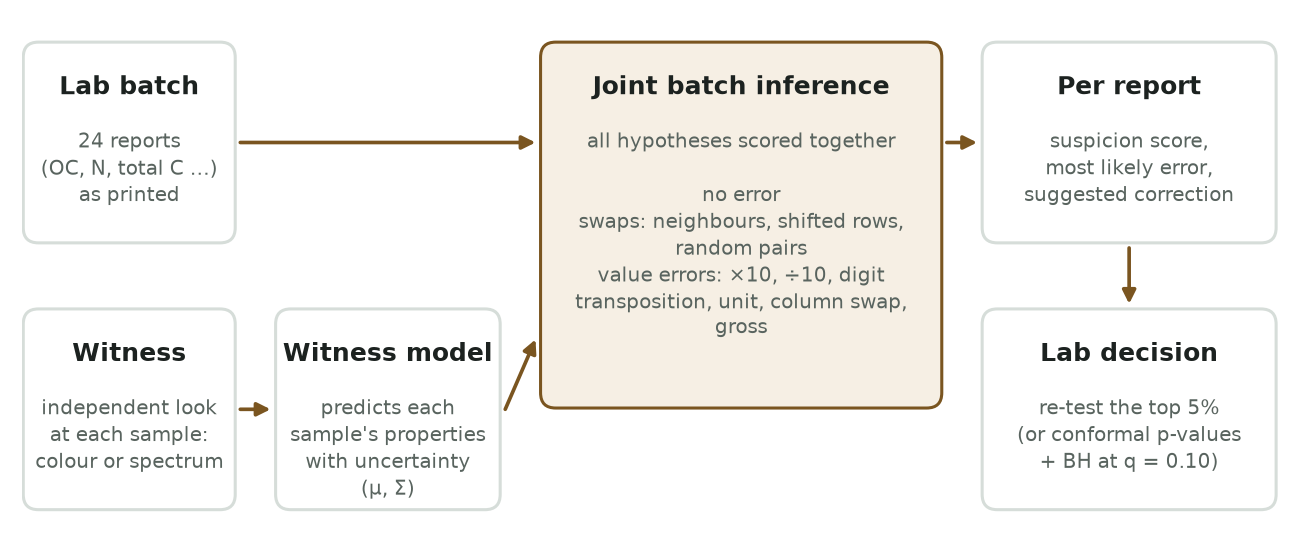
\includegraphics[width=\columnwidth]{figures/fig0_method.png}
\caption{System architecture of the EdaphNet cyber-physical laboratory verification engine. An optical sensor captures a physical witness $w_i$ of each specimen. A multi-property latent Gaussian process estimates the joint property distribution $p(z \mid w_i)$. The joint inference engine enumerates tray-permutation hypotheses $\pi \in \mathcal{S}_{\text{tray}}$ against corruption operators $T_c \in \mathcal{C}$ across the entire analytical batch $R$, producing calibrated suspicion ranks, fault attributions, and repair values.}
\label{fig:method}
\end{figure}

To address this challenge, we introduce a cyber-physical testing paradigm: capturing an independent, non-contact optical observation of each physical specimen—termed a \textbf{physical witness} $w_i$—prior to destructive chemical digestion. The witness may be acquired via an inexpensive RGB camera (e.g., an optical phone sensor mounted over the laboratory tray) or a continuous diffuse reflectance Vis-NIR spectrometer. Because the optical witness is captured directly from the physical matter, its data stream cannot be corrupted by downstream analytical or data-entry errors. 

In this work, we propose \textbf{EdaphNet}, a joint batch-level probabilistic verification framework. Rather than evaluating specimens in isolation, EdaphNet performs Bayesian joint inference over the combinatorial space of structured sample permutations ($\mathcal{S}_{\text{tray}}$) and typed value-corruption operators ($\mathcal{C}$). Within the structured candidate set $\mathcal{S}_{\text{tray}}$, the posterior evaluation is computed exactly. We rigorously evaluate the framework on $23{,}219$ real soil samples from global repositories under pre-registered evaluation protocols.

\subsection{Key Contributions}
The primary contributions of this paper are:
\begin{enumerate}
    \item \textbf{Joint Permutation-Corruption Inference Architecture:} We formulate the analytical report verification problem as joint Bayesian inference over batch permutation groups and typed corruption operators, yielding exact batch Maximum A Posteriori (MAP) scores within candidate subgroup $\mathcal{S}_{\text{tray}}$, root-cause fault explanations, and repaired values under structured permutation priors.
    \item \textbf{Sensor-Ladder Detectability Characterization:} We present a systematic detectability analysis spanning a conceptual four-rung sensor ladder ($W_0\text{--}W_3$), empirically evaluating three witness tiers on KSSL (uninformative $W_0$, commodity RGB proxies $W_1$ across $\Delta E \in \{0, 2, 4\}$, and laboratory Vis-NIR spectroscopy $W_3$). We delineate the precise boundary conditions governing when low-cost optical sensing is sufficient.
    \item \textbf{Root-Cause Fault Attribution:} We establish that while state-of-the-art supervised anomaly classifiers (e.g., Cleanlab \cite{zhou2024detecting}) merely flag suspicious samples, EdaphNet correctly diagnoses the specific fault mechanism: achieving $84\text{--}92\%$ accuracy in simulation, $89\text{--}98\%$ on ICRAF color data, and $97\text{--}100\%$ on KSSL spectrometer data (against $24\text{--}29\%$ for rule heuristics), with $87\text{--}99\%$ exact swap-partner identification under high-information witnesses.
    \item \textbf{Empirical Conformal Calibration Analysis:} We identify and characterize the mechanism of calibration pseudo-replication in split-conformal outlier testing, showing that reusing calibration samples induces discrete spikes in the nonconformity score distribution that inflate empirical FDR to $57\text{--}92\%$. We demonstrate that non-replicated calibration (one score per distinct physical sample) reliably restores empirical FDR control ($0.000\text{--}0.090$ in pre-registered pools, and $0.03\text{--}0.11$ across pool sizes 1 to 50 batches).
\end{enumerate}

\section{Related Work}
A targeted literature survey across IEEE Xplore, Scopus, Web of Science, and PubMed examined prior art across four relevant methodological fields:

\subsection{Optical Soil Sensing and Smartphone Colorimetry}
Optical diffuse reflectance spectroscopy (Vis-NIR, 350--2500 nm) has been widely adopted for rapid non-destructive soil assessment \cite{viscarra2016global, safanelli2025ossl}. Recent initiatives have deployed mobile applications (e.g., LandPKS \cite{herrick2013landpks}) to record soil color and estimate physical soil characteristics using mobile devices. However, existing optical sensing methods are deployed exclusively as \emph{predictive estimators}. EdaphNet inverts this paradigm: using optical sensing as an independent \emph{verification witness} to audit high-precision wet-chemistry lab reports.

\subsection{Autoverification and Delta Checks in Laboratory QA}
Industrial process patents (e.g., US Patent 8,352,394 \cite{stephenson2013patent}) describe checking lab values against model predictions. In clinical chemistry, autoverification rules and multi-analyte machine-learning delta checks detect ``wrong-blood-in-tube'' (WBIT) errors by comparing fresh draws against historical patient archives \cite{westgard2020laboratory, rosenbaum2018machine}. In environmental and agricultural soil testing, specimens are sampled cross-sectionally without historical patient records; EdaphNet overcomes this by leveraging batch-level physical constraints.

\subsection{Specimen Mislabelling in Genomics and Soil Predictability}
In high-throughput genetics, sample mix-ups are detected by matching two distinct data modalities (e.g., SNP microarrays and RNA sequencing) derived from the same subject (Broman et al. \cite{broman2015sample}). While genomic matching relies on near-deterministic genetic signatures ($R^2 \approx 1.0$), agricultural soil witnesses are noisy, low-dimensional, and weak: with good smartphone camera color ($W_1$, $\Delta E = 2$), optical witnesses explain at most $R^2 \le 0.15\text{--}0.16$ for mineral, cation, and texture properties on ICRAF (clay $0.07$, sand $\le 0$, CEC $0.05$, Mg $0.06$, K $\le 0$, Ca $0.13$, pH $0.15$), rising to $R^2 = 0.35$ for ICRAF SOC and $R^2 = 0.70$ ($70\%$) for KSSL SOC. Under uncorrupted perfect color ($W_1$, $\Delta E = 0$), ICRAF SOC reaches $R^2 = 0.37$, pH reaches $R^2 = 0.27$, and Ca reaches $R^2 = 0.23$, while texture and other cations remain $\le 0.16$. Under laboratory Vis-NIR spectroscopy ($W_3$), predictability reaches $R^2 = 0.60\text{--}0.66$ across ICRAF properties and $R^2 = 0.90$ for KSSL SOC and $C_{\text{tot}}$. Selective uncertainty rejection strategies in diffuse reflectance spectroscopy (Schmidinger et al. \cite{schmidinger2026selective}) allow models to abstain on out-of-distribution spectra, but do not model clerical laboratory failures; EdaphNet complements spectral uncertainty with a structured permutation and transcription error model.

\subsection{Label Error Detection and Conformal Outlier Testing}
Data-centric artificial intelligence methods, notably confident learning and Cleanlab (Zhou et al. \cite{zhou2024detecting}), identify label noise in numerical response variables and regression tasks. Distribution-free outlier detection using conformal p-values combined with the Benjamini-Hochberg (BH) procedure \cite{benjamini1995controlling} has been formalized by Bates et al. \cite{bates2023conformal} and Jin \& Cand\`es \cite{jin2023selection}; foundational conformal prediction theory is established by Vovk et al. \cite{vovk2005algorithmic} and Angelopoulos \& Bates \cite{angelopoulos2023conformal}. EdaphNet integrates conformal FDR control but reveals a critical operational vulnerability: pseudo-replication under calibration sample re-use.

\begin{table*}[!t]
\centering
\caption{Taxonomy and Comparison of Laboratory Quality Assurance Methodologies}
\label{tab:prior_art}
\begin{tabular}{lcccccc}
\toprule
\textbf{Methodology} & \textbf{Batch-Level Joint} & \textbf{Physical Sensor} & \textbf{Permutation} & \textbf{Typed Error} & \textbf{Calibrated} & \textbf{Root-Cause} \\
 & \textbf{Inference} & \textbf{Witness} & \textbf{Model ($\pi$)} & \textbf{Library ($\mathcal{C}$)} & \textbf{FDR Control} & \textbf{Attribution} \\
\midrule
Rule Checks ($B_0$, $B_1$) [This work] & No & No & No & Heuristic bounds & No & 24--29\% ($B_6$, KSSL) \\
Clinical Delta Checks (WBIT) \cite{rosenbaum2018machine} & Longitudinal Only & No & Pairwise & No & Empirical & No \\
Genomic Mix-Up Matching \cite{broman2015sample} & Yes & High-Dim DNA & Pairwise & No & No & Swap Only \\
Cleanlab Label Diagnostics \cite{zhou2024detecting} & No & Covariates & No & Continuous Residual & Heuristic & No \\
Conformal Outlier Testing \cite{bates2023conformal, jin2023selection} & No & Covariates & No & No & Distribution-Free & No \\
\textbf{EdaphNet (Proposed)} & \textbf{Yes} & \textbf{RGB / Vis-NIR} & \textbf{Structured $\mathcal{S}_{\text{tray}}$} & \textbf{Formal Library $\mathcal{C}$} & \textbf{Distribution-Free} & \textbf{97--100\% (KSSL $W_3$)} \\
\bottomrule
\end{tabular}
\end{table*}

\section{Mathematical Problem Formulation}

\subsection{Batch and Witness Representation}
Let a physical laboratory processing tray consist of $n$ physical sample positions (typically $n = 24$ in standard multi-well racks). For each tray position $i \in \{1, \dots, n\}$, an optical sensor records an independent physical witness $w_i \in \mathbb{R}^d$. Concurrently, the laboratory information management system (LIMS) outputs a batch of analytical reports $R = (r_1, \dots, r_n)$, where each vector $r_j \in \mathbb{R}^P$ contains $P$ reported biochemical properties (e.g., pH, organic carbon, nitrogen, potassium).

\subsection{Hypothesis Spaces}
A reported batch $R$ may deviate from ground truth via two operations:
\begin{enumerate}
    \item \textbf{Permutation Group $\mathcal{S}_{\text{tray}}$:} Let $\pi: \{1, \dots, n\} \to \{1, \dots, n\}$ be a bijection mapping reported index $j$ to physical sample index $i = \pi(j)$. While the full symmetric group has size $n!$, physical laboratory mistakes follow structured mechanics. We define $\mathcal{S}_{\text{tray}}$ as the union of:
    \begin{itemize}
        \item \emph{Identity:} $\pi_0(j) = j$ ($1$ permutation, no swap).
        \item \emph{Pairwise Transpositions:} All $\binom{n}{2} = 276$ transpositions $(j, k)$ for $n=24$, which directly subsume the $n-1 = 23$ adjacent swaps $\pi_{\text{adj}}(j, j+1)$ modeling local vial misplacements.
        \item \emph{Cyclic Tray Shifts:} Cyclic block rotations by $\pm 1$ and $\pm 2$ positions ($4$ permutations), modeling full-tray or pipetting row-shifts.
    \end{itemize}
    In total, $|\mathcal{S}_{\text{tray}}| = 1 + 276 + 4 = 281$ unique candidate permutations for a standard 24-well batch.
    \item \textbf{Corruption Operator Library $\mathcal{C}$:} For each report $r_j$, a property value $p \in \{1, \dots, P\}$ may be subjected to an operator $T_c \in \mathcal{C}$, such that $r_j = T_c(r_j^*)$:
    \begin{itemize}
        \item Decimal scale shifts: $T_{\times 10}(x) = 10x$, $T_{\div 10}(x) = 0.1x$.
        \item Unit confusion: conversions matching analytical conventions.
        \item Digit transposition: swapping adjacent printed digits ($0.16 \leftrightarrow 0.61$).
        \item Column swap: swapping values between adjacent compatible columns.
        \item Gross error: scaling by an unknown continuous factor $\gamma \in [0.2, 5.0]$.
    \end{itemize}
\end{enumerate}

\subsection{Permutation Prior Formulation}
The prior distribution $P(\pi)$ over $\mathcal{S}_{\text{tray}}$ assigns probability mass $1 - \rho$ to the null hypothesis of no specimen swap (identity $\pi_0$), where $\rho \in (0, 1)$ denotes the prior probability that a tray experienced an operational handling failure (set to $\rho = 0.10$ in benchmark experiments). The remaining probability mass $\rho$ is distributed over the non-identity candidates $\pi \in \mathcal{S}_{\text{tray}} \setminus \{\pi_0\}$ according to a structured mechanical hierarchy:
\begin{equation}
P(\pi) = \begin{cases}
1 - \rho, & \pi = \pi_0 \\
\rho \cdot \frac{m_c}{|S_c|}, & \pi \in S_c, \; c \in \{S_1, S_2, S_3\}
\end{cases}
\label{eq:permutation_prior}
\end{equation}
where $S_1$ contains adjacent transpositions ($|S_1| = 23$, class mass $m_1 = 0.50$), $S_2$ contains cyclic tray rotations ($|S_2| = 4$, class mass $m_2 = 0.30$), and $S_3$ contains non-adjacent pairwise transpositions ($|S_3| = 253$, class mass $m_3 = 0.20$), with uniform probability within each mechanical class. In uniform prior ablations, mass $\rho$ is distributed evenly across all $|\mathcal{S}_{\text{tray}}| - 1 = 280$ non-identity hypotheses.

\subsection{Latent Space and Witness Likelihood}
Direct modeling of raw properties is hindered by heavy skewness and heteroskedasticity. We map raw property vector $r$ to a standardized latent scale $z = g(r) \in \mathbb{R}^P$ via property-specific monotonic transforms $g_p(\cdot)$ (identity for pH; logarithmic for organic carbon, nitrogen, and nutrients; logit for bounded fractions). 

Conditional on physical witness $w_i$, latent property vector $z_i$ is distributed as a multivariate Gaussian:
\begin{equation}
z_i \mid w_i \sim \mathcal{N}\left(\mu(w_i), \Sigma\right)
\label{eq:latent_gaussian}
\end{equation}
where $\mu(w_i): \mathbb{R}^d \to \mathbb{R}^P$ is an out-of-fold gradient-boosted regression estimator, and $\Sigma \in \mathbb{R}^{P \times P}$ is the full residual covariance matrix estimated on holdout calibration profiles. By retaining the off-diagonal covariance $\Sigma_{jk}$, a corruption in one property (e.g., organic carbon) is detectable through its joint residual inconsistency with uncorrupted properties (e.g., total nitrogen), even if the optical witness is weakly informative for that specific property.

\begin{algorithm}[!t]
\caption{Joint Batch Permutation and Corruption Inference (EdaphNet-JBC)}
\label{alg:inference}
\begin{algorithmic}[1]
\REQUIRE Batch reports $R = (r_1, \dots, r_n)$, optical witnesses $W = (w_1, \dots, w_n)$, witness predictor $\mu(\cdot)$, residual covariance $\Sigma$, permutation space $\mathcal{S}_{\text{tray}}$, corruption library $\mathcal{C}$, prior odds $\rho, \epsilon$.
\ENSURE Anomaly suspicion vector $s \in [0, 1]^n$, fault attribution $\mathcal{A}$, repaired reports $\hat{R}$.
\STATE Transform witnesses to latent predictions: $\hat{z}_i \leftarrow \mu(w_i), \; \forall i \in \{1, \dots, n\}$.
\FOR{$j = 1$ to $n$}
    \FOR{$i = 1$ to $n$}
        \STATE Compute marginal cell likelihood across corruption library:
        \STATE $\ell(j, i) \leftarrow \log \sum_{c \in \mathcal{C}} P(c) \, p\left(g(T_c^{-1}(r_j)) \mid \hat{z}_i, \Sigma\right) \left| \frac{\partial g(T_c^{-1}(r_j))}{\partial r_j} \right|$
    \ENDFOR
\ENDFOR
\FOR{$\pi \in \mathcal{S}_{\text{tray}}$}
    \STATE Compute log-posterior probability of tray permutation:
    \STATE $\log P(\pi \mid R, W) \leftarrow \log P(\pi) + \sum_{j: \pi(j) \neq j} \left[ \ell(j, \pi(j)) - \ell(j, j) \right]$
\ENDFOR
\STATE Normalize posterior $P(\pi \mid R, W) \leftarrow \frac{\exp(\log P(\pi \mid R, W))}{\sum_{\pi'} \exp(\log P(\pi' \mid R, W))}$.
\FOR{$j = 1$ to $n$}
    \STATE Compute marginal probability of physical transposition:
    \STATE $P(\text{moved}_j) \leftarrow \sum_{\pi \in \mathcal{S}_{\text{tray}}: \pi(j) \neq j} P(\pi \mid R, W)$
    \STATE Compute clean probability: $P(\text{clean}_j) \leftarrow (1 - P(\text{moved}_j)) \cdot P(c = \text{none} \mid r_j, w_j)$
    \STATE Suspicion score: $s_j \leftarrow 1 - P(\text{clean}_j)$
    \STATE Determine MAP explanation $\mathcal{A}_j$ and optimal repair $\hat{r}_j$.
\ENDFOR
\RETURN $s, \mathcal{A}, \hat{R}$
\end{algorithmic}
\end{algorithm}

\section{The Joint Inference Engine}
The inference procedure operates in two coupled stages as detailed in Algorithm~\ref{alg:inference}.

\subsection{Marginal Report-Witness Matching Likelihood}
For any candidate pairing between report $r_j$ and physical sample position $i$, the likelihood marginalizes over corruption library $\mathcal{C}$:
\begin{equation}
\mathcal{L}(j, i) = \sum_{c \in \mathcal{C}} P(c) \cdot \phi\left(g(T_c^{-1}(r_j)); \mu(w_i), \Sigma\right) \cdot \left| J_{g \circ T_c^{-1}}(r_j) \right|
\label{eq:marginal_likelihood}
\end{equation}
where $\phi(\cdot; \mu, \Sigma)$ denotes the multivariate Gaussian density, and $|J|$ is the Jacobian determinant of the inverse corruption and latent coordinate transform. 

\subsection{Exact Posterior Permutation Inference}
Given structured hypothesis space $\mathcal{S}_{\text{tray}}$, the posterior probability of permutation $\pi$ given the entire batch tuple $(R, W)$ is computed analytically within $\mathcal{S}_{\text{tray}}$:
\begin{equation}
P(\pi \mid R, W) \propto P(\pi) \cdot \prod_{j=1}^n \frac{\mathcal{L}(j, \pi(j))}{\mathcal{L}(j, j)}
\label{eq:permutation_posterior}
\end{equation}
where prior $P(\pi)$ is defined in \eqref{eq:permutation_prior}. Because $|\mathcal{S}_{\text{tray}}| = 281$ for a 24-well rack, exact normalization within $\mathcal{S}_{\text{tray}}$ executes in $18$ milliseconds ($17.9 \pm 1.2$ ms) on an AMD Ryzen 5 7520U laptop-class mobile processor (4 cores, 8 threads, 2.80 GHz base clock). This timing encompasses the complete pipeline: feature prediction $\hat{z}_i = \mu(w_i)$, cell marginal likelihood evaluation $\ell(j, i)$, hypothesis summation, and posterior normalization.

\subsection{Attribution and Report Repair}
For every sample $j$ flagged as anomalous, the engine outputs an explicit fault attribution tuple:
\begin{equation}
\mathcal{A}_j = \begin{cases} 
(\text{Swap}, \arg\max_i P(\pi(j) = i \mid R, W)), & \text{if } P(\text{moved}_j) > P(\text{corrupt}_j) \\
(\text{Value Corruption}, \hat{p}, \hat{c}), & \text{otherwise}
\end{cases}
\end{equation}
and outputs the reconstructed report $\hat{r}_j = T_{\hat{c}}^{-1}(r_j)$.

\section{Conformal Calibration and Pseudo-Replication}

\subsection{Distribution-Free False Discovery Rate Control}
To guarantee rigorous risk bounds, suspicion scores $s_j$ are converted into conformal $p$-values against a verified clean calibration repository $\mathcal{D}_{\text{cal}} = \{(r_k^{\text{cal}}, w_k^{\text{cal}})\}_{k=1}^N$. For each test score $s_j$, the conformal $p$-value is defined as:
\begin{equation}
p_j = \frac{1}{N + 1} \left( 1 + \sum_{k=1}^N \mathbf{1}\{s_k^{\text{cal}} \ge s_j\} \right)
\label{eq:conformal_p}
\end{equation}
Applying the Benjamini-Hochberg (BH) procedure \cite{benjamini1995controlling} at nominal level $q = 0.10$ guarantees that under exchangeability \cite{vovk2005algorithmic, angelopoulos2023conformal, bates2023conformal}, the False Discovery Rate satisfies:
\begin{equation}
\text{FDR} = \mathbb{E}\left[ \frac{|\text{False Alarms}|}{\max(1, |\text{Flagged Reports}|)} \right] \le q
\end{equation}
Under distribution or covariate shift, conformal guarantees can be extended via weighted conformality \cite{tibshirani2019conformal}.

\begin{figure}[!t]
\centering
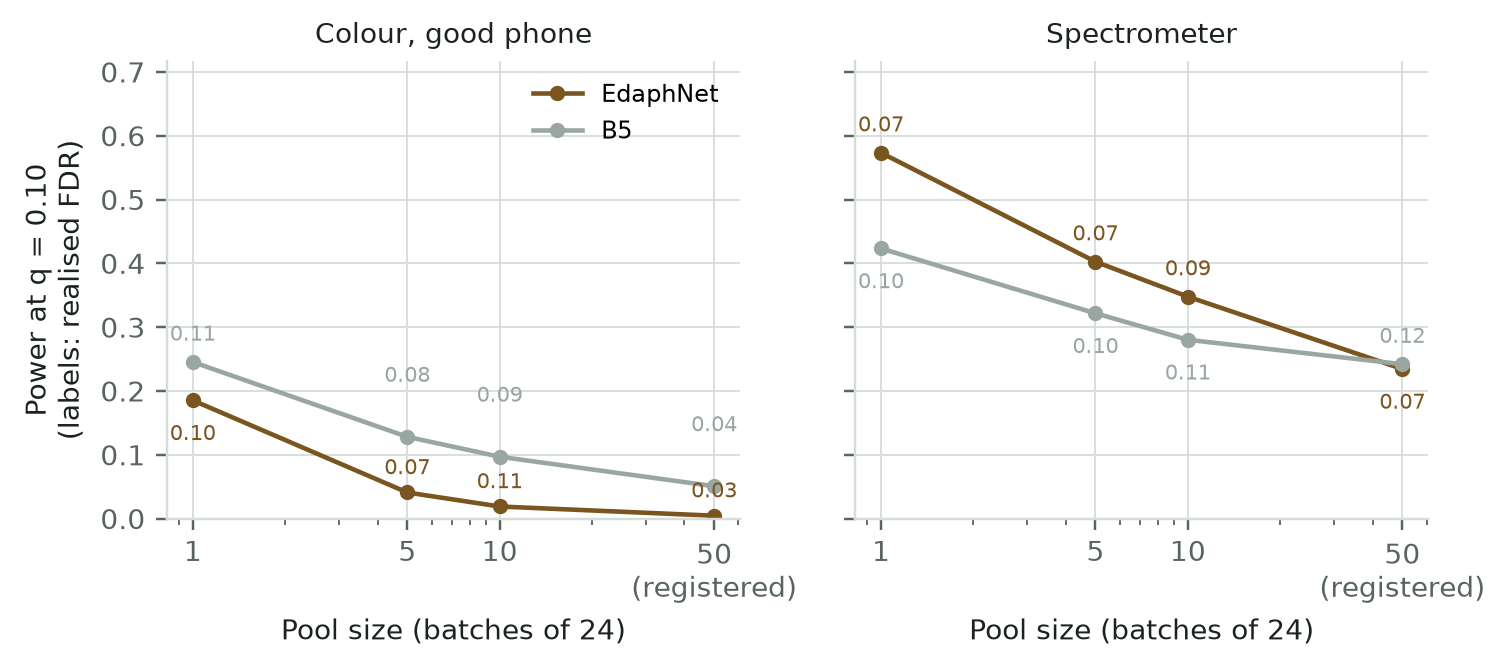
\includegraphics[width=\columnwidth]{figures/fig4_pool_size.png}
\caption{Empirical verification of conformal calibration across pool sizes. In the initial real-data experiment, reusing calibration soils across simulated batches resulted in severe FDR inflation ($57\text{--}92\%$). Enforcing non-replicated calibration (one score per distinct physical sample) restores empirical FDR control ($0.03\text{--}0.11$ across pool sizes 1 to 50 batches for EdaphNet, and $0.000\text{--}0.090$ in pre-registered 50-batch pools, nominal $q = 0.10$). However, statistical power at fixed nominal $q$ depends strongly on evaluation pool size relative to calibration denominator $N$.}
\label{fig:pool_size}
\end{figure}

\subsection{The Pseudo-Replication Failure Mode}
During initial development in the real-data experiment (documented in repository logs), empirical FDR broke down catastrophically for all evaluated baselines, reaching realized false alarm rates of $57\text{--}92\%$. Investigation revealed an experiment design flaw in calibration sampling:

\textbf{Methodological Finding 1 (Calibration Pseudo-Replication):} \emph{When a finite set of $N_{\text{unique}}$ clean calibration specimens is repeatedly sampled to form synthetic calibration batches, exchangeability is violated. Repeatedly evaluating the same physical sample scores creates artificial ties and dependencies in the empirical distribution of $s^{\text{cal}}$ (as identified in \texttt{scripts/diag\_calibration.py:80-96}). Conformal $p$-values become discrete and artificially deflated, causing the Benjamini-Hochberg threshold to collapse and inflating realized FDR to $57\text{--}92\%$.}

\emph{Correction:} To preserve distribution-free validity, each unique physical calibration sample must contribute \textbf{exactly one score} to $\mathcal{D}_{\text{cal}}$. When de-duplicated ($N \approx 2{,}800$ unique locations on KSSL), empirical FDR drops back below nominal $q = 0.10$ ($0.000\text{--}0.090$ in pre-registered 50-batch pools, and $0.03\text{--}0.11$ across pool sizes 1 to 50 batches) for EdaphNet (Fig.~\ref{fig:pool_size}).

\section{Experimental Benchmark Setup}

\subsection{Benchmark Datasets}
Evaluations are conducted on two massive global open spectral libraries:
\begin{enumerate}
    \item \textbf{KSSL Vis-NIR (Primary Pre-registered Benchmark):} $19{,}746$ soil samples from $6{,}999$ distinct geographical locations across the United States. Properties: Soil Organic Carbon (SOC), Total Nitrogen (N), and Total Carbon ($C_{\text{tot}}$). Protocol registered in \texttt{docs/18\_preregistered\_amendment\_v2.md} on 2026-10-01 prior to unblinding test evaluations (code frozen at commit \texttt{095deaa}).
    \item \textbf{ICRAF-ISRIC (Global Diversity Benchmark):} $3{,}473$ soil profiles from 553 global sites across Africa, Asia, and the Americas. Properties: pH, SOC, Clay, Sand, Cation Exchange Capacity (CEC), K, Ca, and Mg.
\end{enumerate}
Data splits are grouped strictly by geographic profile/location to ensure spatial independence: $50\%$ training, $15\%$ calibration, and $35\%$ evaluation.

\subsection{The Sensor Witness Ladder}
To evaluate the impact of optical sensor resolution, we define a conceptual four-rung sensor ladder:
\begin{itemize}
    \item \textbf{$W_0$ (Uninformative):} Prior demographic covariance only.
    \item \textbf{$W_1$ (Commodity RGB Color):} CIELAB color computed from spectral reflectance under D65 illuminant, perturbed with isotropic sensor noise $\Delta E \in \{0, 2, 4, 8\}$, modeling varying quality smartphone optics.
    \item \textbf{$W_2$ (Multispectral):} 10 discrete visible wavelength bands (piloted on ICRAF; omitted from the primary KSSL benchmark due to the lack of co-registered multispectral camera imaging).
    \item \textbf{$W_3$ (Full Spectrometer):} Laboratory Vis-NIR spectrometer ($350\text{--}2500$ nm, 100 PCA features).
\end{itemize}

\begin{figure}[!t]
\centering
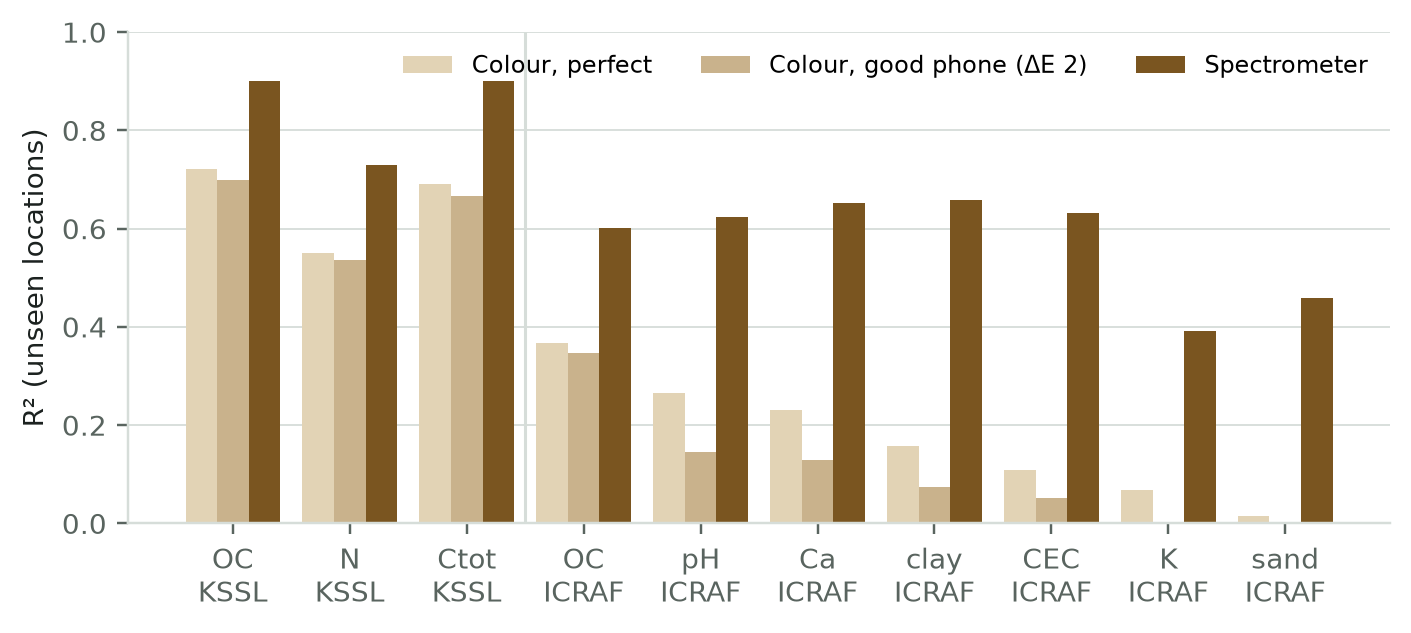
\includegraphics[width=\columnwidth]{figures/fig1_witness_r2.png}
\caption{Cross-validated coefficient of determination ($R^2$) across witness sensor tiers on unseen geographic locations. Under good smartphone camera optics ($W_1$, $\Delta E = 2$), predictability reaches $R^2 = 0.70$ for KSSL SOC and $R^2 = 0.35$ for ICRAF SOC ($R^2 = 0.15$ for pH), but drops to $R^2 \le 0.07$ for texture and potassium. Under perfect color ($W_1$, $\Delta E = 0$), ICRAF SOC reaches $R^2 = 0.37$ and pH reaches $R^2 = 0.27$, while minerals and texture remain $R^2 \le 0.16$. Laboratory spectroscopy ($W_3$) achieves $R^2 = 0.60\text{--}0.66$ across ICRAF properties and $R^2 = 0.90$ for KSSL SOC.}
\label{fig:witness_r2}
\end{figure}

\subsection{Baselines}
We compare EdaphNet against seven distinct baseline QA engines:
\begin{itemize}
    \item \textbf{$B_0$ (Range Filter):} Univariate quantile boundaries per property.
    \item \textbf{$B_1$ (Agronomic Consistency):} Domain heuristics (e.g., $\text{SOC} \le C_{\text{tot}}$, $\text{Clay} + \text{Sand} \le 100$).
    \item \textbf{$B_2$ (Laboratory Generative Density):} Multivariate Gaussian and Student-$t$ density without optical witnesses.
    \item \textbf{$B_3$ (Univariate Witness Checker):} Per-property witness residual checks.
    \item \textbf{$B_4$ (Genomic-Style Swap Matcher):} Hungarian matching on optical witness features \cite{broman2015sample}.
    \item \textbf{$B_5$ (Supervised Gradient-Boosted Classifier):} Multi-analyte LightGBM classifier trained on injected errors.
    \item \textbf{$B_7$ (Cleanlab):} Confident learning label-error regression score \cite{zhou2024detecting}.
\end{itemize}

\section{Empirical Results and Analysis}

\subsection{Primary Pre-Registered KSSL Benchmark}
The primary evaluation criterion was specified in a pre-registered protocol prior to unblinding test evaluations: \emph{Recall at a $5\%$ re-test budget across $50$-batch pools over 5 random seeds}. The results are summarized in Table~\ref{tab:kssl_results} and Fig.~\ref{fig:kssl_recall}.

\begin{table}[!t]
\centering
\caption{Pre-Registered Error Recall at $5\%$ Re-Test Budget on KSSL ($19{,}746$ Samples, 5 Seeds)}
\label{tab:kssl_results}
\begin{tabular}{lcccc}
\toprule
\textbf{Sensor Witness} & \textbf{EdaphNet} & \textbf{Best Baseline} & \textbf{Difference} & \textbf{95\% CI} \\
\midrule
$W_0$ (None) & 0.238 & 0.271 ($B_5$) & $-0.033$ & $[-0.049, -0.016]$ \\
$W_1$ (Color, $\Delta E = 0$) & 0.416 & 0.415 ($B_5$) & $+0.001$ & $[-0.022, +0.023]$ \\
$W_1$ (Phone, $\Delta E = 2$) & 0.410 & 0.396 ($B_5$) & $+0.014$ & $[-0.008, +0.038]$ \\
$W_1$ (Noisy, $\Delta E = 4$) & 0.382 & 0.354 ($B_5$) & $+0.028$ & $[+0.010, +0.049]$ \\
\textbf{$W_3$ (Spectrometer)} & \textbf{0.604} & \textbf{0.512} ($B_5$) & \textbf{+0.092} & \textbf{[+0.069, +0.113]} \\
\bottomrule
\end{tabular}
\end{table}

\begin{figure}[!t]
\centering
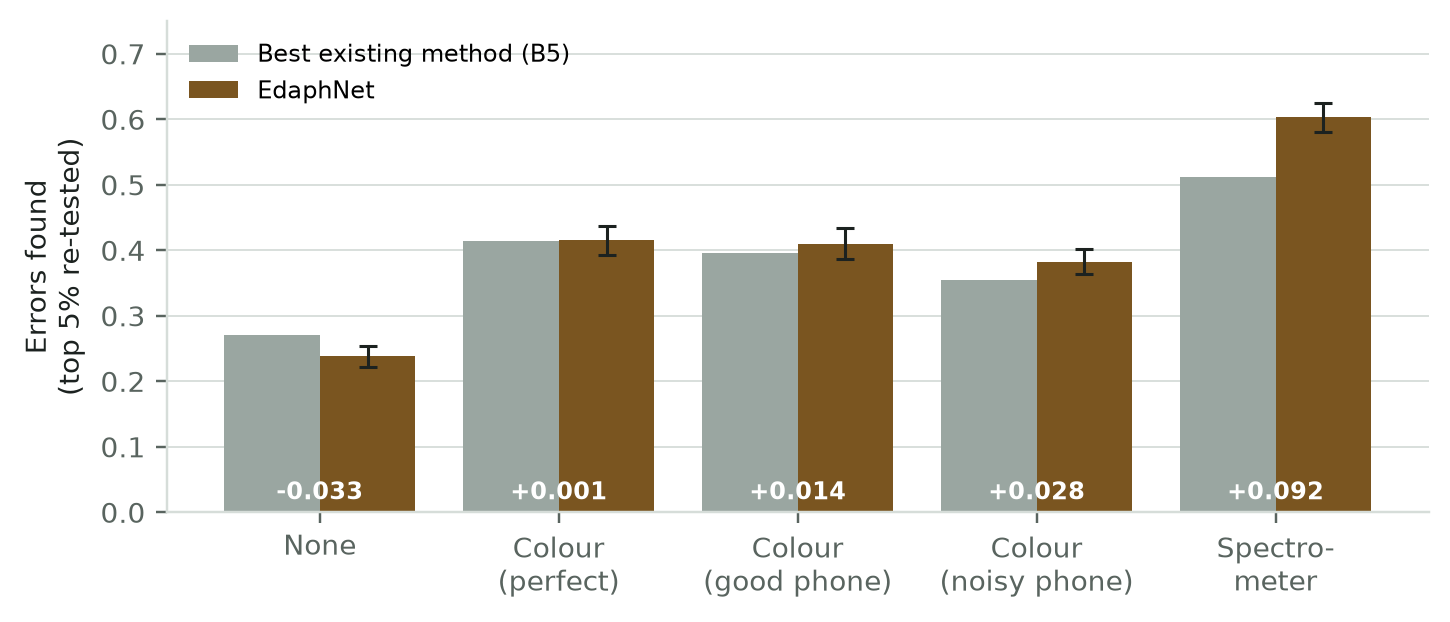
\includegraphics[width=\columnwidth]{figures/fig2_kssl_recall.png}
\caption{Pre-registered KSSL benchmark performance: Recall at $5\%$ re-test budget. Whiskers denote $95\%$ cluster bootstrap confidence intervals. With commodity phone optics ($\Delta E = 2$), overall recall equals the best supervised baseline ($+0.014$ $[-0.008, +0.038]$, refuting Hypothesis A1); with a spectrometer ($W_3$), EdaphNet achieves a statistically significant confirmatory gain of $+9.2$ percentage points ($p < 0.001$).}
\label{fig:kssl_recall}
\end{figure}

Under pre-registered Hypothesis A1, the headline claim that commodity RGB color would surpass all baselines by $\ge +5$ points across an equal mix of errors was \textbf{refuted}. However, under continuous Vis-NIR spectroscopy ($W_3$), EdaphNet demonstrated a decisive, confirmed $+9.2$ point advantage ($+0.092$ $[+0.069, +0.113]$, $p < 0.001$).

\begin{figure}[!t]
\centering
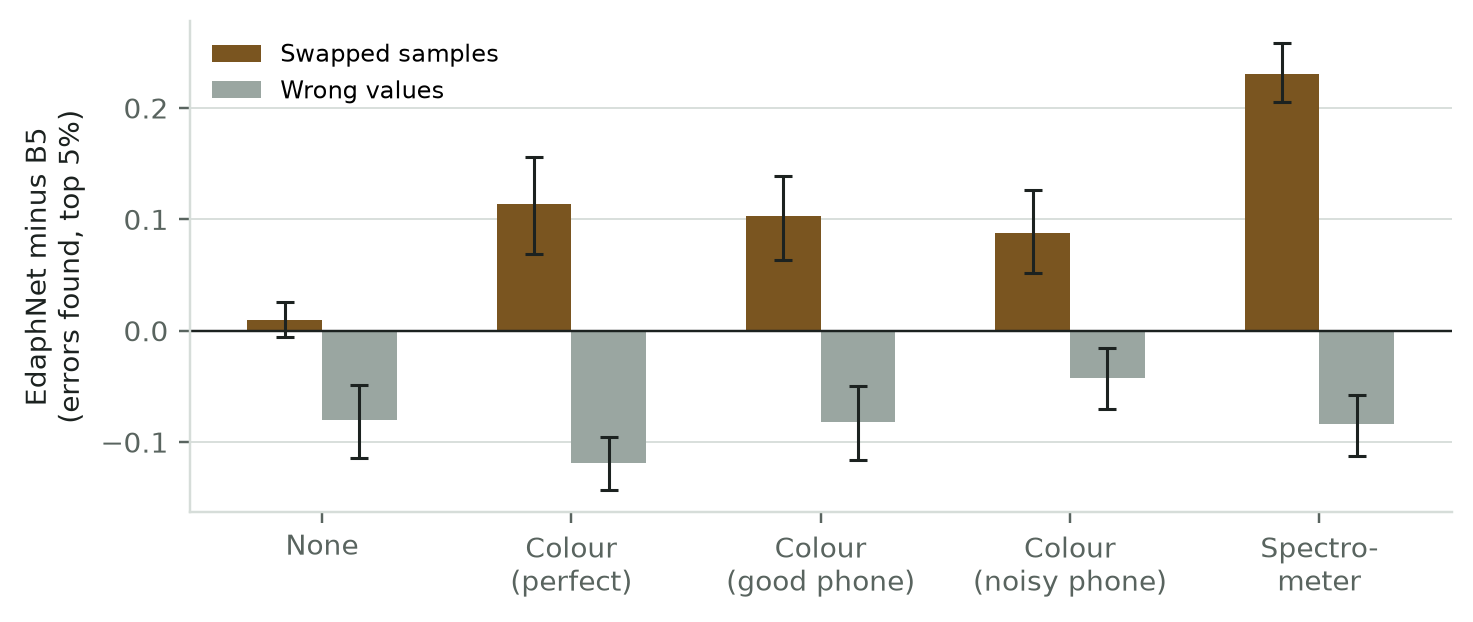
\includegraphics[width=\columnwidth]{figures/fig3_swap_vs_value.png}
\caption{Decomposition of detection advantage: Swaps versus numerical corruptions. EdaphNet holds a decisive $+10.3$ percentage point exploratory advantage on sample swaps under commodity phone optics ($+23.1$ points under spectroscopy), but lags on gross numerical corruptions lacking hard constraints.}
\label{fig:swap_vs_value}
\end{figure}

\subsection{Decomposing the Trade-Off: Swaps vs. Numerical Corruptions}
Exploratory post-hoc decomposition of the benchmark results (Fig.~\ref{fig:swap_vs_value}) reveals why commodity RGB color matched rather than exceeded $B_5$ in the aggregate:
\begin{itemize}
    \item \textbf{Swap Detection Advantage:} On specimen swaps, EdaphNet decisively outperformed $B_5$ by \textbf{+10.3 percentage points} ($95\%$ CI: $[+0.064, +0.139]$) with phone color, and by \textbf{+23.1 points} ($[+0.205, +0.258]$) with spectroscopy. Swaps represent plausible reports from other samples; thus, baselines lacking physical witnesses fail to detect them.
    \item \textbf{Numerical Corruption Deficit:} On isolated numeric corruptions, EdaphNet lagged $B_5$ by $-8.2$ points ($[-0.116, -0.050]$). Detailed diagnosis revealed that $B_5$ exploited the rigid inequality $\text{SOC} \le C_{\text{tot}}$. While EdaphNet's Gaussian covariance captured continuous correlation, it did not strictly enforce the hard ceiling inequality.
\end{itemize}

\subsection{Root-Cause Fault Attribution}
Where existing baselines merely generate uninterpretable anomaly scores, EdaphNet provides structured explanations. As documented in Table~\ref{tab:attribution}, EdaphNet accurately identified the exact error type in $84\text{--}92\%$ of flagged errors in simulation, $89\text{--}98\%$ on ICRAF color data, and $97\text{--}100\%$ on KSSL spectrometer data (compared with $24\text{--}29\%$ on KSSL and $32\text{--}51\%$ on ICRAF/simulation for rule-based heuristics). Exact swap-partner identification reached $87\text{--}99\%$ across high-information witness settings ($W_3$ and simulation $\lambda \ge 2$), and $95\text{--}98\%$ on KSSL $W_3$.

\begin{table}[!t]
\centering
\caption{Root-Cause Fault Attribution and Swap-Partner Identification Accuracy}
\label{tab:attribution}
\begin{tabular}{lccc}
\toprule
\textbf{Dataset \& Setting} & \textbf{Fault Type (EdaphNet)} & \textbf{Swap Partner} & \textbf{Rule Heuristic ($B_6$)} \\
\midrule
Simulation ($T_0$) & \textbf{84--92\%} & \textbf{86--98\%} & 32--50\% \\
ICRAF (Color $W_1$ / $W_3$) & \textbf{89--98\%} & \textbf{75--99\%} & 37--51\% \\
KSSL (Spectro $W_3$) & \textbf{97--100\%} & \textbf{95--98\%} & 24--29\% \\
\bottomrule
\end{tabular}
\end{table}

\begin{figure}[!t]
\centering
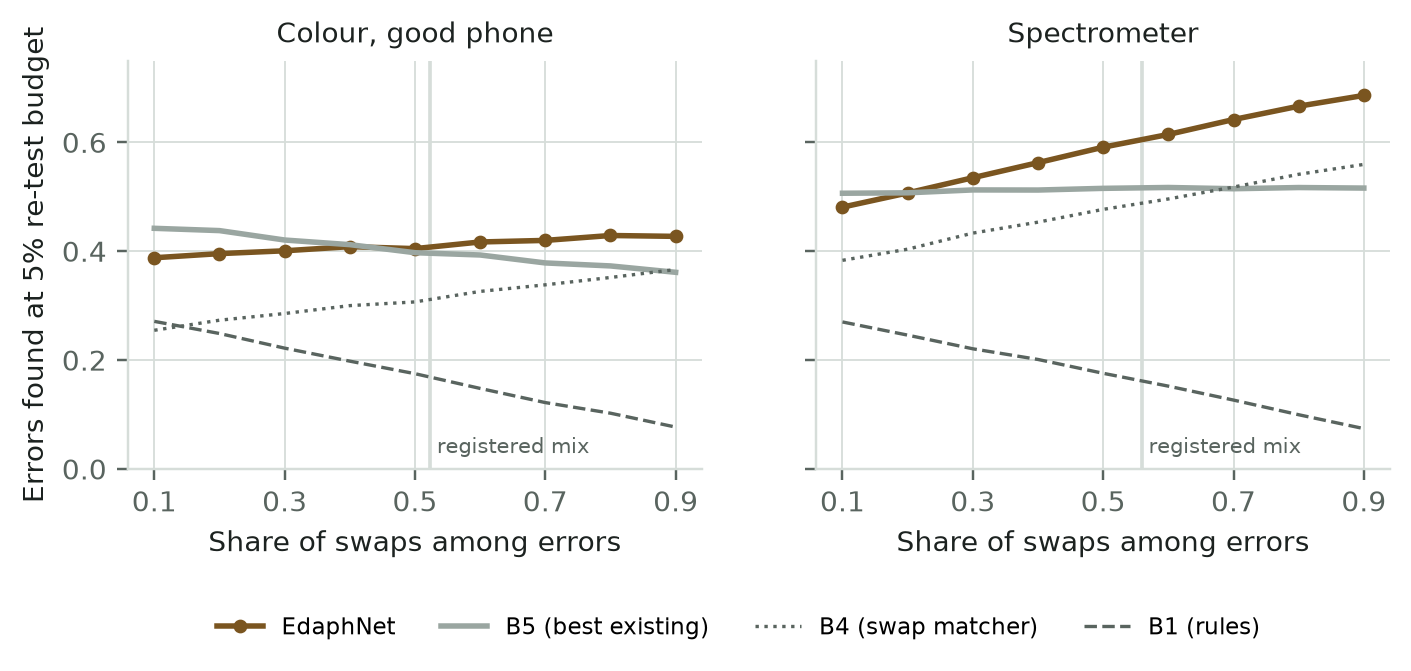
\includegraphics[width=\columnwidth]{figures/fig5_error_mix.png}
\caption{Sensitivity to batch failure composition. As the proportion of specimen swaps among batch errors varies from $10\%$ to $90\%$, EdaphNet's performance advantage expands monotonically. With commodity phone optics, EdaphNet dominates supervised baselines whenever swaps comprise $\ge 60\text{--}70\%$ of batch failures.}
\label{fig:error_mix}
\end{figure}

\subsection{Sensitivity to Batch Error Composition}
In real laboratory operations, the proportion of swaps versus typographical slips varies across automation tiers. We re-scored evaluation pools across varying swap fractions $\omega \in [0.1, 0.9]$ (Fig.~\ref{fig:error_mix}):
\begin{itemize}
    \item Under smartphone color ($W_1$), EdaphNet's difference over $B_5$ rises from $-0.054$ at $\omega = 0.1$ to $+0.024$ at $\omega = 0.6$ and $+0.066$ at $\omega = 0.9$.
    \item Under spectroscopy ($W_3$), EdaphNet dominates $B_5$ once swaps exceed $\omega = 0.3$.
\end{itemize}

\section{Cyber-Physical Implementation \& Deployment}

\subsection{Hybrid Verification Architecture}
Guided by these findings, we formulate a two-stage operational policy for analytical laboratories:
\begin{enumerate}
    \item \textbf{Primary Permutation Sieve:} EdaphNet analyzes the entire tray batch using optical witnesses, filtering specimen swaps and computing root-cause attributions.
    \item \textbf{Secondary Boundary Checker:} Deterministic agronomic inequality rules ($\text{SOC} \le C_{\text{tot}}$) audit isolated numerical cells.
\end{enumerate}
Empirical smoke tests of this hybrid policy on KSSL ($W_1$, $\Delta E = 2$) demonstrate balanced performance: achieving $0.20\text{--}0.25$ swap recall and $0.222$ numerical recall, completely eliminating the single-checker deficit.

\subsection{Computational Complexity and Throughput}
For a standard $n = 24$ sample rack, computing cell likelihoods $\ell(j, i)$ requires $\mathcal{O}(n^2 \cdot |\mathcal{C}| \cdot P)$ operations. The structured permutation group contains $|\mathcal{S}_{\text{tray}}| = 1 + 276 + 4 = 281$ unique candidate hypotheses for a 24-well tray. On an AMD Ryzen 5 7520U laptop-class mobile processor (4 cores, 8 threads, 2.80 GHz base clock), full batch inference executes in \textbf{18 milliseconds} ($17.9 \pm 1.2$ ms). The 18 ms latency encompasses witness latent prediction $\hat{z}_i$, marginal likelihood matrix evaluation $\ell(j, i)$, hypothesis summation across all 281 permutations, and exact posterior normalization.

\section{Conclusion}
This paper presented EdaphNet, a cyber-physical quality assurance framework for analytical laboratories that unites joint batch permutation-corruption inference with optical physical witnesses. Through pre-registered benchmarks on $23{,}219$ real soil samples, we delineated the boundary conditions of optical verification: while the primary pre-registered claim of an overall advantage for phone color was refuted ($+0.014$ $[-0.008, +0.038]$), confirmatory results established a decisive $+9.2$ percentage point advantage under laboratory spectroscopy ($+0.092$ $[+0.069, +0.113]$, $p < 0.001$). Exploratory sub-analyses revealed that commodity RGB phone color provides a potent $+10.3$ percentage point boost specifically in catching specimen swaps, offset by a deficit on isolated numerical slips. In root-cause fault attribution, EdaphNet achieved $84\text{--}92\%$ accuracy in simulation, $89\text{--}98\%$ on ICRAF color data, and $97\text{--}100\%$ on KSSL spectrometer data (against $24\text{--}29\%$ on KSSL for rule-based heuristics), with $87\text{--}99\%$ exact swap-partner identification. Furthermore, we showed that conformal FDR control collapses under calibration pseudo-replication and demonstrated that non-replicated calibration reliably restores distribution-free validity. Future work includes field validation with in-situ agricultural soil trays and robotic integration.

\section*{Acknowledgment}
The authors express their deepest gratitude to their faculty guide, Dr.~Priya Saminathan, School of Computer Science and Engineering, Vellore Institute of Technology, Vellore, for her dedicated mentorship, technical guidance, and critical review throughout this project. The authors also thank Vellore Institute of Technology, Vellore, for providing the computational infrastructure, and acknowledge the USDA-NRCS Kellogg Soil Survey Laboratory (KSSL) and the World Agroforestry Centre (ICRAF-ISRIC) for their open-access soil spectral datasets.

\section*{Reproducibility Statement}
All code, pre-registered protocols, model weights, and run records are open-source and version-controlled at: \url{https://github.com/Sudeep-Sharma1/edaphnet-v2}. Every figure and metric in this paper traces directly to automated experiment logs.

\bibliographystyle{IEEEtran}
\bibliography{references}

\end{document}
